%%%%%%%%%%%%%%%%%%%%%%%%%%%%%%%%%%%%%%%%%
% baposter Landscape Poster
% LaTeX Template
% Version 1.0 (11/06/13)
%
% baposter Class Created by:
% Brian Amberg (baposter@brian-amberg.de)
%
% This template has been downloaded from:
% http://www.LaTeXTemplates.com
%
% License:
% CC BY-NC-SA 3.0 (http://creativecommons.org/licenses/by-nc-sa/3.0/)
%
%%%%%%%%%%%%%%%%%%%%%%%%%%%%%%%%%%%%%%%%%

%----------------------------------------------------------------------------------------
%	PACKAGES AND OTHER DOCUMENT CONFIGURATIONS
%----------------------------------------------------------------------------------------

\documentclass[landscape,a0paper,fontscale=0.285]{baposter} % Adjust the font scale/size here

\usepackage{graphicx} % Required for including images
\graphicspath{{figures/}} % Directory in which figures are stored

\usepackage{amsmath} % For typesetting math
\usepackage{amssymb} % Adds new symbols to be used in math mode
%\usepackage[czech]{babel}
\usepackage[utf8x]{inputenc}
\usepackage{psfrag,graphicx}
\usepackage{fancybox,color,colortbl}
\usepackage{float, picinpar}
\usepackage{multicol}
\usepackage{amsmath}
\usepackage{epstopdf}

\usepackage{booktabs} % Top and bottom rules for tables
\usepackage{enumitem} % Used to reduce itemize/enumerate spacing
\usepackage{palatino} % Use the Palatino font
\usepackage[font=small,labelfont=bf]{caption} % Required for specifying captions to tables and figures

\usepackage{multicol} % Required for multiple columns
\setlength{\columnsep}{1.5em} % Slightly increase the space between columns
\setlength{\columnseprule}{0mm} % No horizontal rule between columns

\usepackage{tikz} % Required for flow chart
\usetikzlibrary{shapes,arrows} % Tikz libraries required for the flow chart in the template

\newcommand{\compresslist}{ % Define a command to reduce spacing within itemize/enumerate environments, this is used right after \begin{itemize} or \begin{enumerate}
\setlength{\itemsep}{1pt}
\setlength{\parskip}{0pt}
\setlength{\parsep}{0pt}
}

\definecolor{lightblue}{rgb}{0.145,0.6666,1} % Defines the color used for content box headers

\begin{document}

\begin{poster}
{
headerborder=closed, % Adds a border around the header of content boxes
colspacing=1em, % Column spacing
bgColorOne=white, % Background color for the gradient on the left side of the poster
bgColorTwo=white, % Background color for the gradient on the right side of the poster
borderColor=lightblue, % Border color
headerColorOne=black, % Background color for the header in the content boxes (left side)
headerColorTwo=lightblue, % Background color for the header in the content boxes (right side)
headerFontColor=white, % Text color for the header text in the content boxes
boxColorOne=white, % Background color of the content boxes
textborder=roundedleft, % Format of the border around content boxes, can be: none, bars, coils, triangles, rectangle, rounded, roundedsmall, roundedright or faded
eyecatcher=true, % Set to false for ignoring the left logo in the title and move the title left
headerheight=0.1\textheight, % Height of the header
headershape=roundedright, % Specify the rounded corner in the content box headers, can be: rectangle, small-rounded, roundedright, roundedleft or rounded
headerfont=\Large\bf\textsc, % Large, bold and sans serif font in the headers of content boxes
%textfont={\setlength{\parindent}{1.5em}}, % Uncomment for paragraph indentation
linewidth=2pt % Width of the border lines around content boxes
}
% \begin{frame}[fragile]
\begin{columns}[T]
% #############################################################################
% #############################################################################
% #############################################################################
% First Column
\begin{column}{.33\textwidth}

\begin{block}{Filter Bubble}
    \center
    \begin{large}\textbf{Living in one's own information environment.}\end{large}
    \vspace{0.8cm}
    \begin{itemize}
        \item occures on social networks
        \item caused by preferential algorithms
        \item first mentioned by Eli Pariser (2011)
    \end{itemize}
\end{block}
% #############################################################################
\begin{block}{Twitter}
	\begin{itemize}
		\item microblogging platform
        \item \textbf{following, followers} system
		\item Twitter API is suitable data source
	\end{itemize}
	\center
	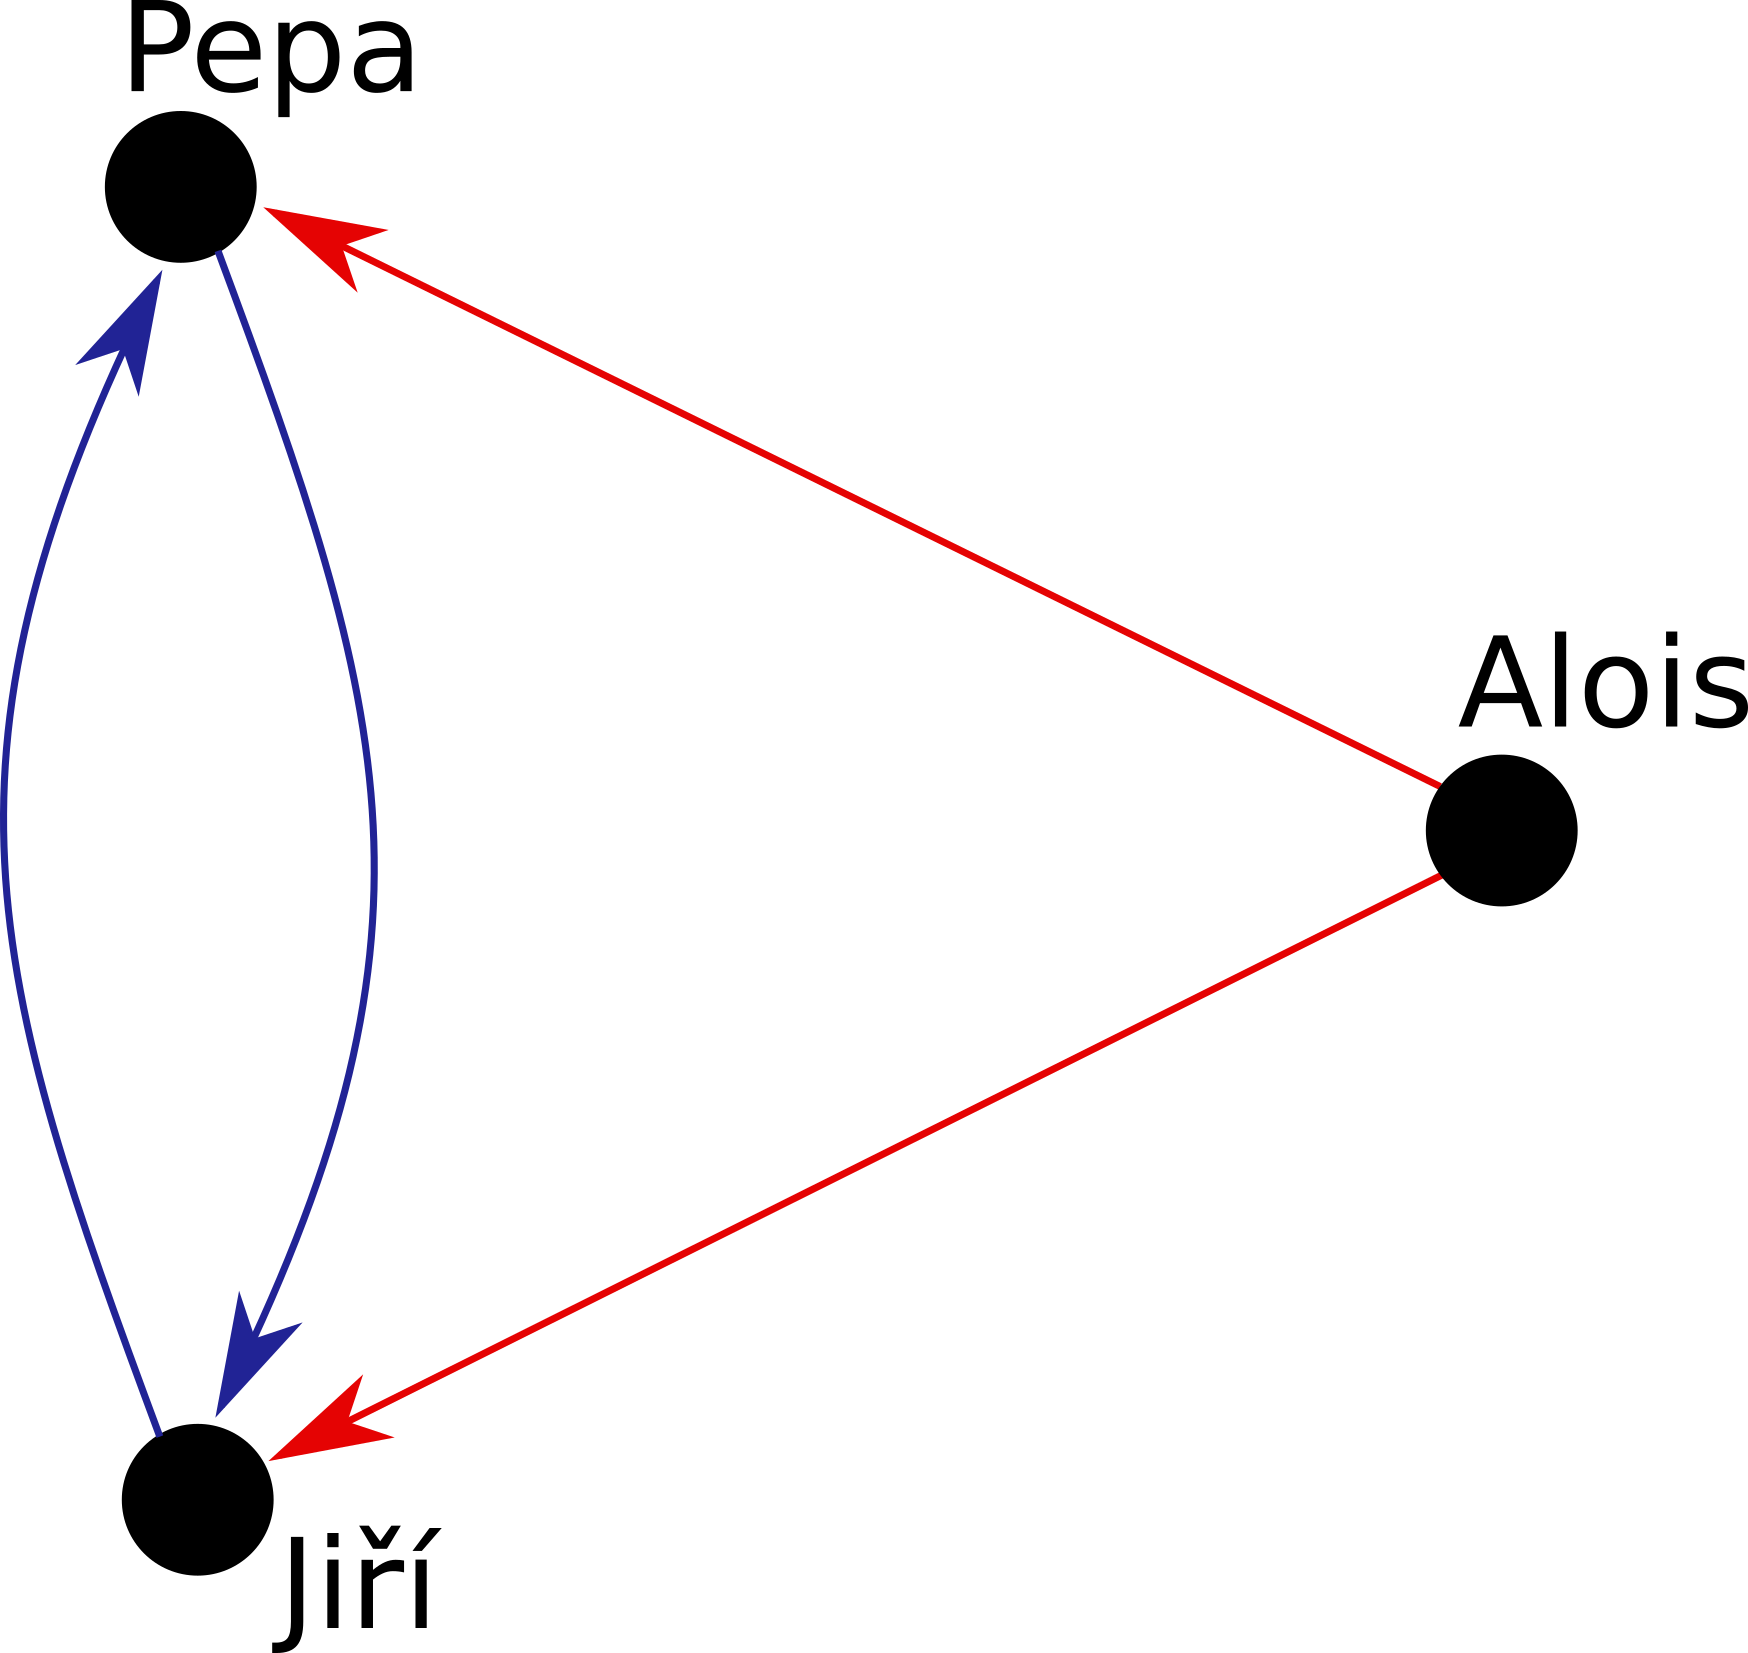
\includegraphics[scale=0.55]{./Pics/pepa.png}
\end{block}
% #############################################################################
\begin{block}{Studied groups selection}
    \begin{columns}
        \begin{column}{.5\textwidth}
            \begin{itemize}
                \item random sample from followers of the significant group
            \end{itemize}
        \end{column}
        \begin{column}{.5\textwidth}
            \center
            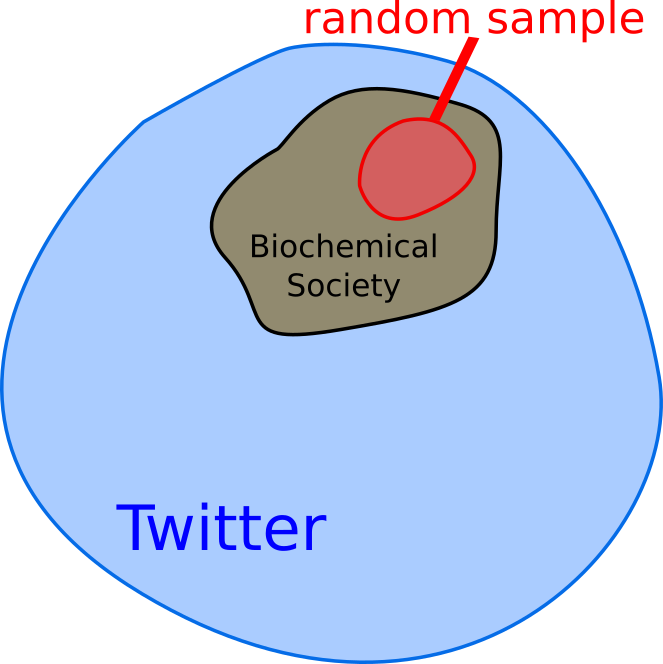
\includegraphics[scale=0.45]{./Pics/sets.png}
        \end{column}
    \end{columns}
    \center
    $\text{Twitter} \rightarrow \text{Biochemical Society} \rightarrow \text{\textbf{studied people}}$
\end{block}
% #############################################################################
\begin{block}{Tweets collection}
    \begin{columns}
    \column{.5\textwidth}
    	\begin{itemize}
            \item analysing content affecting the studied people
    	\end{itemize}
    \column{.5\textwidth}
    	\center
    	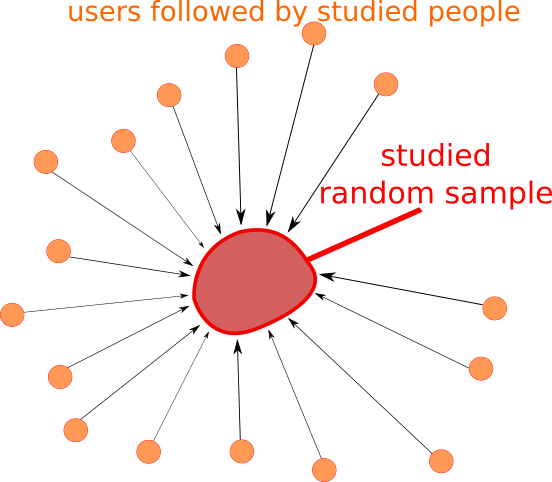
\includegraphics[scale=0.65]{./Pics/followers.png}
    \end{columns}
    \vspace{0.8cm}
    \begin{itemize}
        \item i. e. content from \textbf{followed people}
    \end{itemize}
\end{block}
% #############################################################################
\begin{block}{Tweets filtering}
\begin{itemize}
    \item filter only tweets on given topic
\end{itemize}
\vspace{0.3cm}
Keyword \textbf{"Trump"}:
\vspace{0.7cm}
\begin{itemize}\centering
    \item[\textcolor{black}{\xmark}] I had fish and chips for lunch.
    \item[\textcolor{black}{\cmark}] I'm glad Donald \textbf{Trump} is the president of the USA.
    % \item[\textcolor{black}{\xmark}] The president of the USA is a gentleman.
\end{itemize}
\end{block}
% #############################################################################
\begin{block}{Sentimental analysis}
\begin{itemize}
    \item measure sentiment of collected tweets
    \item \textbf{positive} vs. \textbf{negative} tweets
\end{itemize}
\center
\textit{Donald Trump is a terrible person.}\\
\textbf{(0.14)}\\
\vspace{0.5cm}
\textit{Donald Trump is a great person.}\\
\textbf{(0.95)}
\end{block}

\end{column}
% #############################################################################
% #############################################################################
% Second Column
\begin{column}{.63\textwidth}
    \begin{customalertblock}{Motivation}
        \begin{columns}
            \begin{column}{.5\textwidth}
                \begin{large}\textbf{Threats for democracy:}\end{large}
                \vspace{0.5cm}
                \center
                content \textbf{homogeneity}\\
                $\Downarrow$\\
                loss of objectivity\\
                $\Downarrow$\\
                \textbf{radicalization}
            \end{column}
            \begin{column}{.5\textwidth}
                \begin{large}\textbf{Goals:}\end{large}
                \vspace{0.5cm}
                \begin{itemize}
                    \item filter bubble detection
                    \item filter bubble quantification
                \end{itemize}
            \end{column}
        \end{columns}
    \end{customalertblock}
\end{column}
\end{columns}
% #############################################################################
% #############################################################################
% #############################################################################








% \begin{columns}[T]
% % #############################################################################
% % #############################################################################
% % #############################################################################
% % First Column
% \begin{column}{.33\textwidth}
%
% \end{column}
% % #############################################################################
% % #############################################################################
% % #############################################################################
% % Second Column
% \begin{column}{.3\textwidth}
%
% \end{column}
% % #############################################################################
% % #############################################################################
% % #############################################################################
% % Third column
% \begin{column}{.33\textwidth}
%
% \end{column}
% % #############################################################################
% % #############################################################################
% % #############################################################################
% \end{columns}

% \end{frame}
\end{poster}

\end{document}
